\subsubsubsubsection{Stretch decorator}
\begin{figure}[h]
\centering
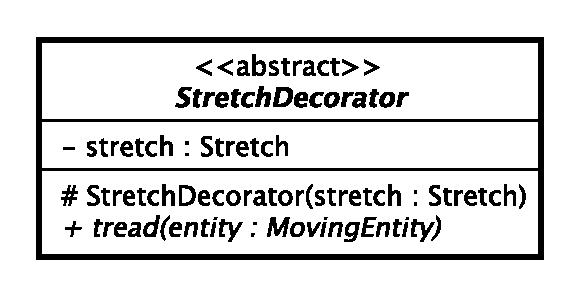
\includegraphics[scale=0.6,keepaspectratio]{images/solution/app/backend/stretch_decorator.eps}
\caption{\pReactiveComponentStretchDecoration::StretchDecorator}
\label{fig:sd-app-stretch_decorator}
\end{figure}
\FloatBarrier
\begin{itemize}
  \item \textbf{\descr} \\
    It represents the abstract decorator which enable to compose togheter several
behaviours on the top of a stretch component. 
  \item \textbf{\attrs}
  \begin{itemize}
    \item \texttt{stretch: Stretch} \\
The stretch to decorate.
  \end{itemize}
  \item \textbf{\ops}
   \begin{itemize} 
   \item[\#] \texttt{StretchDecorator(stretch: Stretch)} \\
Creates a stretch decorator with a specific stretch to decorate.
    \item[+] \texttt{\textit{tread(entity: MovingEntity)}} \\
Decorates the standard behaviour of the stretch.  
  \end{itemize}
\end{itemize}
